%
\section{Domain Behaviour Semantics} \label{sect:arch-module-actions}
Using the unified model at the core of a MOSA model requires defining for the modules a set of essential actions for manipulating the domain objects of a domain class.
%
We consider these actions as forming a module interface, which is represented by a UML interface named  \clazz{ModuleService}.
In this section, we provide a formal definition of module action, which is suitable for use with the activity graph language that we propose in Section~\ref{sect:agl}. Our definition focuses on describing the structure of module action and its pre- and post-states. We base our formalism on the UML Action language (\S{16}\footnote{We use `\S{}' to denote both Chapter and Section, which is interpreted from the context.}~\cite{omg_unified_2015}), which incorporates the notion of state. State is argued to be an intrinsic part of behavioral specification (\S{14}~\cite{omg_unified_2015}).
%
We recursively define module action by beginning with the most primitive type of action called \textit{atomic action}. We then combine these actions to form \textit{atomic action sequence} and, more generally, \textit{structured atomic action}.
% 
\subsection{Expressing Domain Behaviour with UML Activity Diagram}
behavior -> activity

behavior structure -> control and action nodes

We focus on providing the semantics for Action.

\subsection{Module-Based Action Semantics}
% TODO: explain the mapping from Action to Module Action

%\subsection{A Formalism for Module Action} 
%
\subsubsection{Atomic Action} \label{sect:arch-atomic-action}
Although each module is different, we observe that there exists a set of primitive behaviours that underlie all modules. We capture these primitive behaviours in what we term \textit{atomic actions}.
%
\begin{definition} \label{def:atomic-action}
An \textbf{atomic action} is a smallest meaningful module behavior provided to a user (which is either a human or another module/system) through the view for manipulating the domain objects of the domain class.

%
Atomic action is characterised by: 
\begin{itemize}
\item \membern{name}: the action name.
%
\item \membern{preStates} (for \membern{localPrecondition}~\cite{omg_unified_2015}): the states at which a current module must be in in order for this action to proceed.
%
\item \membern{postStates} (for \membern{localPostcondition}~\cite{omg_unified_2015}): the states at which the action completes its execution on a current module.
%
\item \membern{fieldValSet} (for \membern{input}~\cite{omg_unified_2015}): captures the input of the action. It is a set of pairs $(f,v)$ where $f$ is name of a domain field of the domain class and $v$ is the value that is to be set to this field by the action. 
%
\item \membern{output}: the domain class for object manipulation actions and empty for all other actions.

Although attribute \membern{name} uniquely identifies an action, for ease of exposition, we usually list two other attributes, \membern{postStates} and \membern{fieldValSet}, with \membern{name}.
%
Thus, we denote by $ a = (o,s,i) $ an atomic action $a$ whose \membern{name}, \membern{postStates} and \membern{fieldValSet} are $ o $, $ s $ and $i$ (\resp). We use the dot notation to refer to the components, \eg $ a.\membern{postStates} = s$.
\end{itemize} \qed
\end{definition}

Note the followings about the above definition. 
First, we use module states to abstract from the local pre- and post-conditions of each action. This abstraction enables us to flexibly combine actions based on states to construct more complex ones. A \textbf{module state} abstracts from the states of the model, view and controller components of a module as these components handle a module action. Certain module states can occur concurrently, resulting in what we call \textbf{concurrent state}s. We write these states using the operator `+'. 
The \membern{postStates} of primitive action consists of a single state, while that of more complex actions (discussed in Section~\ref{sect:arch-saa}) consists of multiple states.

Second, because each action concerns manipulating the values of some domain fields of the domain class, the action inputs, if any, need to be those that are used for updating these fields. Thus, we define action inputs as a (possibly empty) field-value set. An element of this set is a pair $(f,v)$, where $f$ is a field name and $v$ is a value. The value $v$ in each pair is either specified by the user or from another action that has previously been performed. The latter case occurs when we compose actions together to form more complex behavior. We will explain action composition in the subsequent subsections.
%We look up the fields using field names and use  their data types as types of the input parameters of the action.

%
Third, the action output consists of at most one type, which is the domain class of the current module. Further, only the object manipulation actions have this output; other actions have an empty output because they do not produce any real output value.

% TODO: + atomic action
% + open: preStates = {Init}
\begin{table}[ht]
	\setlength\tabcolsep{1pt}
	\centering
	\footnotesize
	\caption{The core atomic actions}\label{tab:core-atomic-actions}
	\begin{tabular}{|>{\centering\arraybackslash}m{2.7cm}|>{\centering\arraybackslash}m{5.6cm}|>{\centering\arraybackslash}m{1.9cm}|>{\raggedright\arraybackslash}m{4.8cm}|}
		%content
		\hline
		\rowcolor{lightgray}
		\textbf{Name} & \textbf{Pre-states}  & \textbf{Post-states} & \textbf{Description} \\\hline
		\membern{open} & \{\code{Init}\} & \{\code{Opened}\} & Open the module's view presenting the domain class. \\\hline
		\membern{newObject} & \{\code{Opened}, \code{Created}, \code{Updated}, \code{Reset}, \code{Cancelled}\} & \{\code{NewObject}\} & Remove from the view any object currently presented and prepare the view for creating a new object. \\\hline
		\membern{setDataFieldValues} & \{\code{NewObject}, \code{Editing}, \code{Created}, \code{Updated}, \code{Reset}, \code{Cancelled}\} & \{\code{Editing}\} & Set values for a sub-set of the view's data fields. \\\hline
		\membern{createObject} & \{\code{NewObject}, \code{Editing} + \code{ObjIsNotPresent}\} & \{\code{Created}\} & Create a new object from data entered on the view. The created object is presented on the view.\\\hline
		\membern{updateObject} & \{\code{Editing} + \code{ObjIsPresent}\} & \{\code{Updated}\}& Update the current object from data entered on the view. The updated object remains on the view.\\\hline
		\membern{deleteObject} & \{\code{Created}, \code{Updated}, \linebreak \code{Reset} + \code{ObjIsPresent}, \linebreak \code{Cancelled} + \code{ObjIsPresent}\} & \{\code{Deleted}\} & Delete the current object. The deleted object is removed from the view.\\\hline
		\membern{reset} & \{\code{Editing}\} & \{\code{Reset}\} & Initialise the view to redisplay the current object (discarding all user input).\\\hline
		\membern{cancel} & \{\code{NewObject}, \code{Editing} + \code{ObjIsNotPresent}\} & \{\code{Cancelled}\} & Cancel creating a new object (discarding all user input, if any).\\\hline
	\end{tabular}
\end{table}

%
Table~\ref{tab:core-atomic-actions} lists definitions of the core atomic actions. %
For exposition purpose, we divide the actions into two groups. %
The first group includes actions that concern the overall operational context of the module.
The actions in this group include \membern{open}, \membern{newObject}, \membern{setDataFieldValues}, \membern{reset} and \membern{cancel}. The post-states of these actions consist of the following states: \code{Opened}, \code{NewObject}, \code{Editing}, \code{Reset} and \code{Cancelled} (\resp). 
%
The second group include three essential domain object manipulation actions: \membern{createObject}, \membern{updateObject} and \membern{deleteObject}. The post-states of these actions include the following states: \code{Created}, \code{Updated} and \code{Deleted} (\resp).
%
%We will illustrate the atomic actions in various examples that will be presented later in this paper.

Note from Table~\ref{tab:core-atomic-actions} that only action \membern{setDataFieldValues} requires the \membern{fieldValSet} to be specified as input. Other actions do not require any input and thus, for them, this set is empty. Note also how the two module states \code{ObjIsPresent} and \code{ObjIsNotPresent} can each occur concurrently with any one of the following states: \code{Editing}, \code{Reset} and \code{Cancelled}. For example, the concurrent state \code{Editing} + \code{ObjIsPresent} means that the module is currently presenting an object on the view and that this object is being edited by the user. In contrast, \code{Editing} + \code{ObjIsNotPresent} means that the module is currently prompting the user to enter input data for a new object. This object has not yet been created.
%
\subsubsection{Atomic Action Sequence (ASE)} \label{sect:arch-ase}
In practice, the core atomic actions are combined in sequence to form more useful behavior. This behavior, which we call \textit{atomic action sequence}, corresponds with an interaction scenario. We model this sequence using structured action of UML activity diagram (\S{16.11}~\cite{omg_unified_2015}).
%
Denote by $ \func{first}$ and $ \func{last}$ two functions that return the first and last elements (\resp) in a sequence.
%
\begin{definition} \label{def:ase}
An \abbrv{atomic action sequence}{ASE} $S = (a_1,\dots,a_n)$ is a module action iff $a_i.\membern{postStates} \subseteq a_{i+1}.\membern{preStates} ~(\forall a_i, a_{i+1} \in S)$.

$S$ has the following properties:
\begin{itemize}
\item $S.\membern{preStates} = \func{first}(S).\membern{preStates}$
\item $S.\membern{postStates} = \func{last}(S).\membern{postStates}$ 
\item $S.\membern{fieldValSet} = \func{first}(S).\membern{fieldValSet}$
\item $S.\membern{output} = \func{last}(S).\membern{output}$ 
\end{itemize}
%
\qed
\end{definition}

%
\begin{figure}[ht]
	\centering
	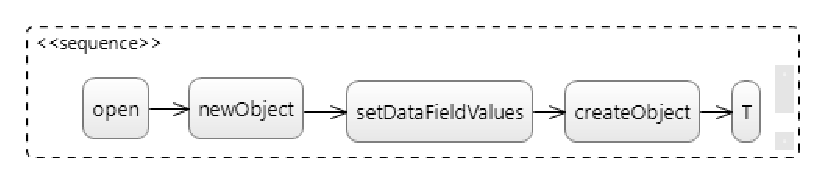
\includegraphics[scale=0.35]{ase-example}
	\caption{An ASE that creates a new domain object of a module's domain class (typed $T$) .} %
	\label{fig:ase-example}
\end{figure}

For example, Figure~\ref{fig:ase-example} shows an ASE that creates a new domain object whose type is the domain class $T$ of a module. This ASE consists in a sequence of four atomic actions and is characterised by:

 \membern{name} = \strq{Sequence:~create~objects}, \membern{postStates} = \{ \code{Created} \} and

 \membern{fieldValSet} = \attrib{setDataFieldValues}{fieldValSet} = $\emptyset$.

The first atomic action is \membern{open}, which opens the view presenting the domain class. Once completed, this action raises an event with the state \code{Opened}, so that interested listeners of this event can handle. This action then leads to the execution of the second atomic action: \membern{newObject}. This sequence is valid because, as listed in Table~\ref{tab:core-atomic-actions}, \attrib{open}{postStates} $\subset$ \attrib{newObject}{preStates}. Action \membern{newObject} prepares the view so that it is ready to receive input from the user for creating a new object. Once completed, this action raises an event with state \code{NewObject}.
%
Because this state is contained in \attrib{setDataFieldValues}{preStates}, we place \membern{setDataFieldValues} as the third action of the ASE. This action is responsible for setting the values of all the view fields, which render the domain fields of the domain class.
Finally, because \attrib{setDataFieldValues}{postStates} $\subset$ \attrib{createObject}{preStates} we place \membern{createObject} as the next (and final) action of the ASE. This action creates a new domain object (using values of the view fields).

A useful property that emerges from our notion of ASE is that there exists a natural multi-level nesting of ASE-backed behaviours along a path in the module containment tree. More specifically, an ASE $S$ is `nested' inside another ASE $S'$ if there exists an activity edge that connects a member action of $S'$ to the start action of $S$. In MOSA, $S'$ is performed on the view of a composite module, and $S$ is on the view of one of its child modules.
%
For example, the ASE of \clazz{ModuleStudent} (shown in Figure~\ref{fig:ase-example}) has a nested ASE which is performed on the child module of type \clazz{ModuleEnrolment}. The ASE of \clazz{ModuleStudent} itself is nested inside that of \clazz{ModuleSClass}, thereby creating a 2-level nesting.
%
\subsubsection{Reachable States} \label{sect:arch-reachable-states}
The definition of ASE gives rise to a notion of \textit{reachable state}, which is a module state that is reachable from a given action. We discuss this notion below and use it in the subsequent subsection to define a more generic action composition.
%
\begin{definition} \label{def:reachable-state}
A module state $s'$ is \textbf{reachable} from an atomic action $a$ if there exists at least one ASE whose first member action is $a$ and whose post-state is $s'$. Action $a$ is called the \textbf{source action} of $s'$. \qed
\end{definition}

%
\begin{table}[ht]
	\setlength\tabcolsep{1pt}
	\centering
%	\footnotesize
	\caption{The core atomic actions and their reachable states}\label{tab:reachable-states}
	\begin{tabular}{|>{\centering\arraybackslash}m{4cm}|>{\arraybackslash}m{12cm}|}
		%content
		\hline
		\rowcolor{lightgray}
		\textbf{Actions} & \textbf{Reachable states} \\\hline
		\membern{open} & \code{Opened}, \code{NewObject}, \code{Editing}, \code{Created}, \code{Updated}, \code{Deleted}, \code{Reset}, \code{Cancelled}\\\hline
		\membern{newObject} & \code{NewObject}, \code{Editing}, \code{Created}, \code{Reset}, \code{Cancelled}\\\hline
		\membern{setDataFieldValues} & \code{Editing}, \code{Created}, \code{Updated}, \code{Reset} \\\hline
		\membern{createObject} & \code{Created} \\\hline
		\membern{updateObject} & \code{Updated} \\\hline
		\membern{deleteObject} & \code{Deleted} \\\hline
		\membern{reset} & \code{Reset} \\\hline
		\membern{cancel} & \code{Cancelled} \\\hline
	\end{tabular}
\end{table}

Clearly, the post-state of an atomic action is reachable from its own action. Table~\ref{tab:reachable-states} lists the reachable states of every atomic action defined in Table~\ref{tab:core-atomic-actions}.
The first row shows how action \membern{open} can reach all other states. This is because once the module's view is opened, it is ready to perform any of the core atomic actions (in some sequences).
The rest of the core actions cannot reach state \code{Opened}, because this state is raised only once.
The second row shows how action \membern{newObject} additionally cannot reach \code{Updated} and \code{Deleted}. This is because this action is reserved for creating a new object. It thus cannot also lead to updating or deleting an existing object.
The third row shows how action \membern{setDataFieldValues} cannot reach \code{NewObject}, \code{Deleted} and \code{Cancelled}. This is because this action concerns only with inputting data and thus cannot initiate or cancel object creation, nor can it lead to object deletion.
%
The last five rows of the table show that the corresponding five actions each has only one reachable state, which are their own states. These actions are ``stubs'', in the sense that they terminate all the ASEs that lead to them.

For example, the ASE in Figure~\ref{fig:ase-example} shows that state \code{Created} is reachable from any of the three member actions that precedes the action \membern{createObject}. These include \membern{open}, \membern{newObject} and \membern{setDataFieldValues}. 
%
\subsubsection{Structured Atomic Action (SAA)} \label{sect:arch-saa}
More generally, we observe that a set of related ASEs form a \textit{structured atomic action}. In essence, this action defines a generic behavior that consists of alternative interaction scenarios (each of which is specified by one ASE in the set) that are usually performed (possibly concurrently) by the user.
%
\begin{definition} \label{def:saa}
	A \abbrv{structured atomic action}{SAA}, \wrt a source atomic action $ a $ and a set of post-states $ E = \{ s_{1},\dots,s_{n} \} $ reachable from $a$, is the set $ A = \{S ~|~ \func{first}(S) = a, S.\attribn{postStates} \subseteq E \} $, where:
  \begin{itemize}
  \item $A.\membern{preStates}$ = $a.\attribn{preStates}$
  \item $A.\membern{postStates}$ = $E$
  \item $A.\membern{fieldValSet}$ = $a.\attribn{fieldValSet}$
  \item $A.\membern{output}$ = $\bigcup_{S \in A} (S.\attribn{output})$
  \end{itemize}

  Abstractly, we write $ A = (a, \{ s_{1},\dots,s_{n} \}, i) $. If $i$ = $\emptyset$ then we omit it and simply write $A$ as $(a, \{ s_{1},\dots,s_{n} \})$. \qed
\end{definition}

Clearly, SAA generalises both atomic action and ASE: an ASE is a single-member SAA, while an atomic action $ a $ is the SAA $ (a, \{ a.\membern{postState} \}, a.\membern{fieldValSet}) $. Further, SAA is significantly shorter to compose than an ASE set -- all we need to do is specify the start atomic action and the desired post-states. 

For example, let us consider the SAA $ (\code{newObject}, \{ \code{Created},\code{Cancelled} \}) $, which represents a common ASE set that starts with action \membern{newObject} and ends only when either the state \code{Created} or the state \code{Cancelled} is detected. The ASE set consists of the following frequently-occurring ASEs. The 
first ASE is the one described earlier in Figure~\ref{fig:ase-example} but excludes the first action. We assume here that the module's view is already opened. The remaining ASEs model alternative scenarios in which the user wants to cancel creating the object at some point between performing the \membern{newObject} action and the \membern{createObject} action.
%
%\subsubsection{Discussion} \label{sect:module-act-discussion}
%We wish to stress that our definition of module action incorporates the notion of state, which is more formally modelled in another UML behavioral modeling language called Behaviour State Machines (BSM) (\S{14.2}~\cite{omg_unified_2015}). The reason that this is possible is because Activity diagram and BSM are tightly linked insofar as behavior is tightly linked to state and state transition. Indeed, these languages represent two sides of the same coin: the former emphasises the actual behavior, while the latter focuses on the behavior's effects (states and state transitions). More specifically, a close inspection of the BSM's abstract syntax (\S{14.2.2}) reveals that both \clazz{State} and \membern{Transition} have associated \clazz{Behaviour}(s) that describe what actually takes place when a particular state is reached or during a transition between some two states.
%Our notion of module action's pre- and post-states simply looks at the same view but from the behavior's perspective.

%A key difference in our definition of module action, however, is that we allow for a more flexible high-level behavior specification (see Definition~\ref{def:saa}), in which a behavior may terminate at not at most one (as implied in the BSM's specification (\S{14.2.2})) but multiple states. Of course, such a behavior may not terminate freely at any states. In our definition, we precisely specify which reachable states can be used to terminate a module action.